% \documentclass[../../Orator]{subfiles}
\documentclass[class={.NoTouch/myProject}, crop=false]{standalone}
\IfStandalone{%
    \import{}{customCommands}
    \import{}{INP-00-glossary}
    }{}
    
    
\begin{document}



\section{The inspiration}

\section{Input}
\indent Since we want want minimize the effects of a possible bias in our data, it makes sense to use the Gaussian white noise signal as an input. But why? \newline

\indent Gaussian white noise is a stationary and ergodic random process with zero mean. Considering an ergodic process is useful in a sense that one can infer meaningful statistics of the process given only that same process. Having a zero mean will just make the data analysis even simpler as well since the model will describe  only the fluctuations of the input received by a neuron.

\textbf{Ergodic process:} the expected value of an observable A is not dependent on time and its time average converges to its value(the average behavior over time is the same as the average potential behavior at a point in time).

\begin{figure}[h]
    \centering
    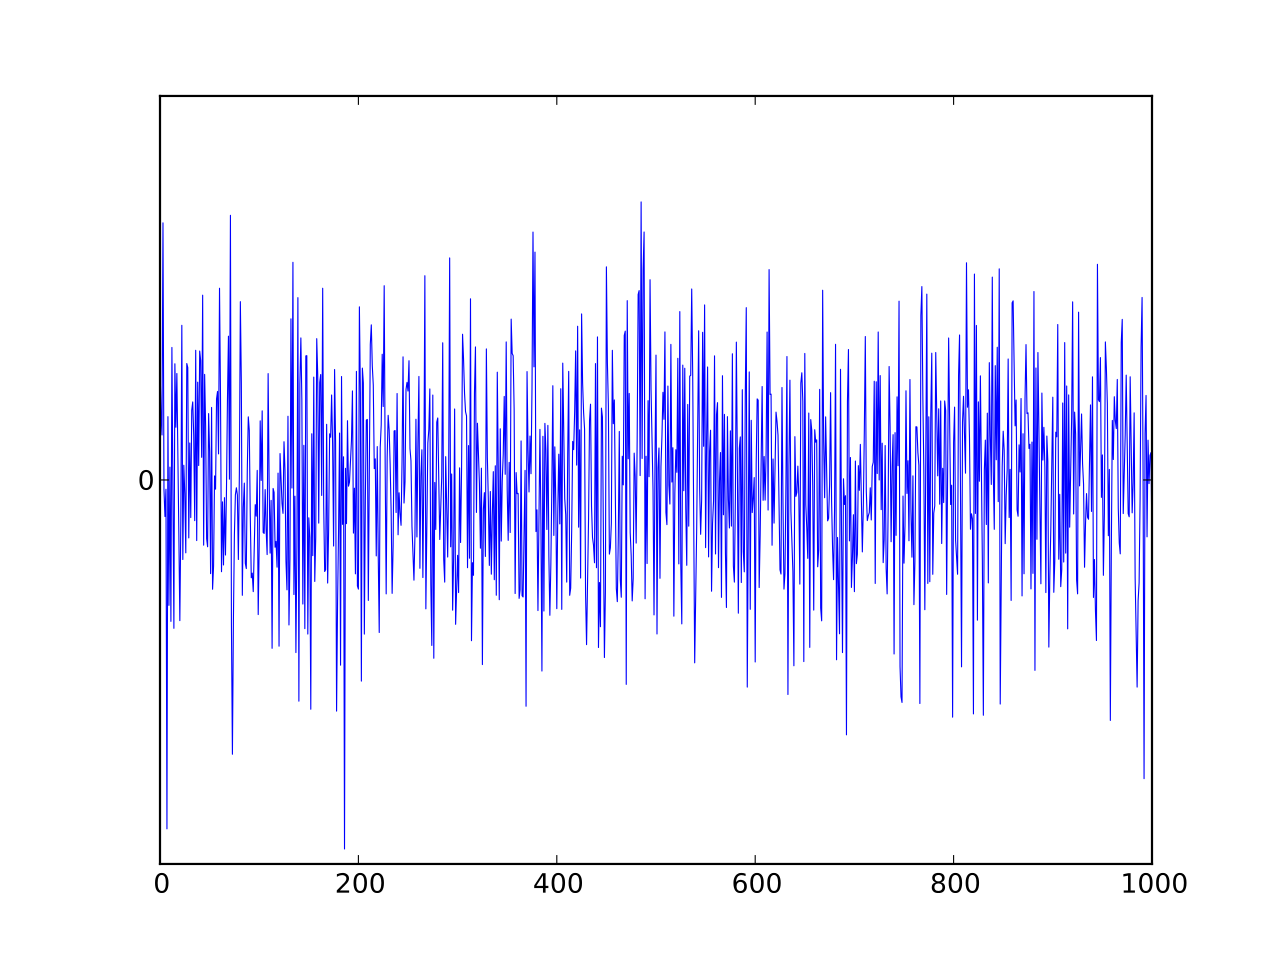
\includegraphics[width=300 pt]{Pictures/Ana/White_noise.svg.png}
    \caption{The waveform of a Gaussian white noise signal plotted on a graph \cite{}.} \label{fig:unkown}
\end{figure}
\section{Neuronal Motif}

\indent Effectively studying the dynamics of neurons becomes very complex in big systems if one takes as basis the Hodgkin-Huxley model. In opposition to this, studying the behaviour of one neuron will not give a reasonable representation of the neuronal dynamics. For this reason, it makes sense to consider small neuronal motives to serve as basis of study for neuronal dynamics while being able to take in consideration the biological characteristics of neurons. Such characteristic network building blocks are also prevalent in biological networks \cite{Sporns2004}

\indent Using nodes to represent neurons in a system, one can consider different types of connections between nodes as in the figure below:


\begin{figure}[h!]
    \centering
    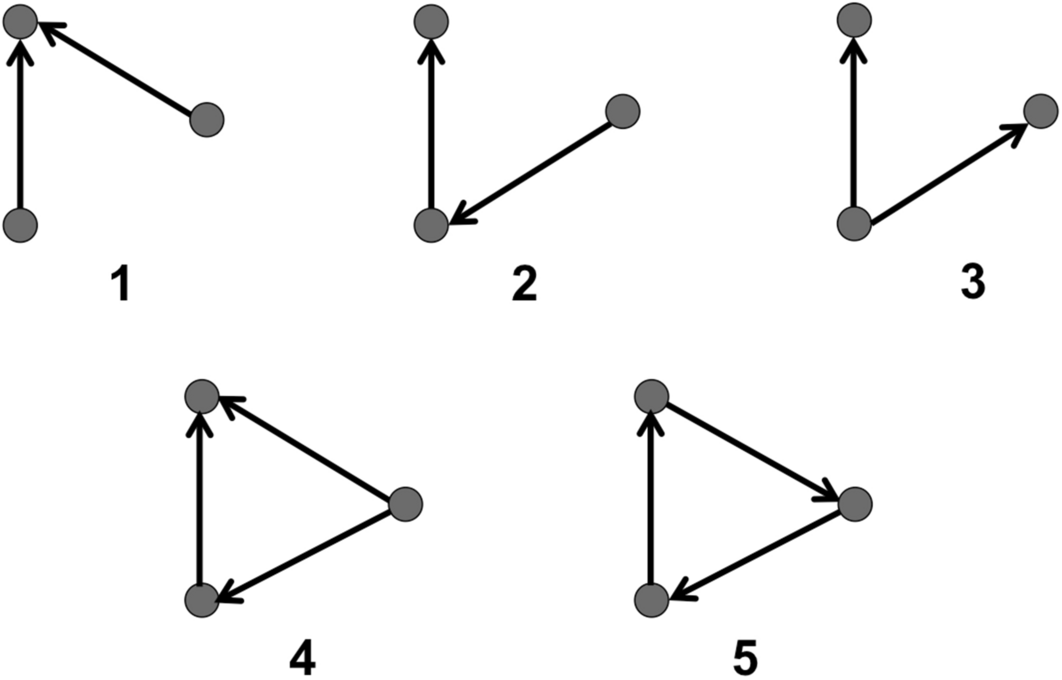
\includegraphics[width=200 pt]{Pictures/Ana/Motif.png}
    \caption{ Possible unidirectional 3-node network motifs. \cite{Shadizadeh2022}}
    \label{fig:enter-label}
\end{figure}

\section{How will these neuronal populations behave?}

Let's take the example of two nodes. \newline

\textbf{Excitatory synapses:}If one connects them mutually with excitatory synapses the two populations will synchronize(more or less depending on external input and the strength of mutual connections).

\textbf{Inhibitory synapses:} If one connects them mutually with inhibitory synapses the two populations will "compete" resulting in one suppressed node and a winner one.

\textbf{Excitatory and inhibitory synapses:} If the nodes are connected by a excitatory and inhibitory synapses, the resulting behaviour will be oscillatory.

UNTIL EACH NUMBER SHOULD I WRITE? WHAT DETAILS WOULD BE NICE?

INSERT FIGURE
TYPES OF MOTIVES(write about their connections)

\end{document}